% !TeX program = xelatex
\documentclass[a4paper,10pt]{article}

% ============================================================================
% សន្លឹកកិច្ចការសិស្ស ស-ខ្មៅ (No-LCD Student Fill-In Worksheet - Grade 8 Lesson 14.2)
% ត្រូវគ្នា ១០០% នឹង LS_Plan_AREA2.tex | ២ ទំព័រ A4 ពេញ (>=90% Page Utilization)
% ============================================================================
\usepackage[a4paper, left=1.0cm, right=1.0cm, top=0.80cm, bottom=1.00cm, footskip=0.50cm]{geometry}
\usepackage{amsmath, amssymb}
\usepackage{unicode-math}
\usepackage{fontspec}
\usepackage{array, colortbl}
\usepackage[table]{xcolor}
\usepackage{enumitem}
\usepackage{pifont}
\usepackage{fancyhdr}
\usepackage{lastpage}
\usepackage{tikz}
\usepackage[most]{tcolorbox}
\usetikzlibrary{calc, arrows.meta, angles, quotes, decorations.markings, positioning, babel}

\makeatletter
\let\@expl@@@mark@update@singlecol@structures@@\relax
\makeatother

\providecommand{\NGSFindFonts}{%
  \IfFileExists{C:/Windows/Fonts/cambria.ttc}{%
    \def\NGSSysPath{C:/Windows/Fonts/}%
    \def\NGSUserPath{C:/Users/KIT/AppData/Local/Microsoft/Windows/Fonts/}%
  }{%
    \IfFileExists{./fonts/KhmerOSsiemreap.ttf}{\def\NGSSysPath{./fonts/}\def\NGSUserPath{./fonts/}}{%
    \IfFileExists{../fonts/KhmerOSsiemreap.ttf}{\def\NGSSysPath{../fonts/}\def\NGSUserPath{../fonts/}}{%
    \IfFileExists{../../fonts/KhmerOSsiemreap.ttf}{\def\NGSSysPath{../../fonts/}\def\NGSUserPath{../../fonts/}}{%
    \IfFileExists{../../../fonts/KhmerOSsiemreap.ttf}{\def\NGSSysPath{../../../fonts/}\def\NGSUserPath{../../../fonts/}}{%
    \IfFileExists{../../../../fonts/KhmerOSsiemreap.ttf}{\def\NGSSysPath{../../../../fonts/}\def\NGSUserPath{../../../../fonts/}}{%
    \IfFileExists{../../../../../fonts/KhmerOSsiemreap.ttf}{\def\NGSSysPath{../../../../../fonts/}\def\NGSUserPath{../../../../../fonts/}}{%
    \IfFileExists{../../../../../../fonts/KhmerOSsiemreap.ttf}{\def\NGSSysPath{../../../../../../fonts/}\def\NGSUserPath{../../../../../../fonts/}}{%
      \def\NGSSysPath{../../../../../../../fonts/}\def\NGSUserPath{../../../../../../../fonts/}%
    }}}}}}}%
  }%
}
\NGSFindFonts

\setmathfont[Path={\NGSSysPath}, FontIndex=1, Scale=1.02]{cambria.ttc}
\defaultfontfeatures{Ligatures=TeX}

\setmainfont[
  Path={\NGSUserPath},
  Extension=.ttf,
  Script=Khmer,
  BoldFont={KhmerOSsiemreap},
  BoldFeatures={FakeBold=1.8},
  ItalicFont={KhmerOSsiemreap},
  ItalicFeatures={FakeSlant=0.25},
  BoldItalicFont={KhmerOSsiemreap},
  BoldItalicFeatures={FakeBold=1.8, FakeSlant=0.25}
]{KhmerOSsiemreap}

\newfontfamily\muol[Path={\NGSUserPath}, Extension=.ttf, Script=Khmer]{KhmerOSmuollight}
\newfontfamily\TimesEn[Path={\NGSSysPath}, Extension=.ttf, BoldFont={timesbd}, ItalicFont={timesi}, BoldItalicFont={timesbi}]{times}

\XeTeXlinebreaklocale "km"
\XeTeXlinebreakskip = 0pt plus 1pt minus 0.1pt

\definecolor{panelgray}{gray}{0.93}
\definecolor{headgray}{gray}{0.85}

\pagestyle{fancy}
\fancyhf{}
\renewcommand{\headrulewidth}{0pt}
\fancyfoot[L]{\fontsize{8.0pt}{10pt}\selectfont អនុវិទ្យាល័យព្រះក្រសាំង \en{|} គណិតវិទ្យា ថ្នាក់ទី៨ \en{|} មេរៀនទី១៤ (១៤.២) ផ្ទៃក្រឡាចតុកោណស្មើ}
\fancyfoot[R]{\fontsize{8.2pt}{10pt}\selectfont ទំព័រ \en{\thepage\ / \pageref{LastPage}}}

\setlength{\parindent}{0pt}
\setlength{\parskip}{0pt}
\setlength{\tabcolsep}{4pt}

\newcommand{\en}[1]{{\TimesEn #1}}
\newcommand{\enbf}[1]{{\TimesEn\bfseries #1}}
\newcommand{\unit}[1]{\,\text{\en{#1}}}
\newcommand{\cnum}[1]{\mbox{\fontsize{10pt}{12pt}\selectfont\ding{\numexpr181+#1\relax}}}
\newcommand{\chkbox}{\tikz[baseline=-0.18ex]\draw[black, line width=0.85pt] (0,0) rectangle (0.26cm,0.26cm);}
\newcommand{\blank}[1]{\makebox[#1]{\dotfill}}
\newcommand{\tri}[1]{\ensuremath{\triangle #1}}
\newcommand{\ang}[1]{\ensuremath{\angle #1}}
\newcommand{\cg}{\ensuremath{\cong}}

\newcommand{\rightbox}[4][0.22cm]{%
  \draw[black, line width=0.8pt]
    ($(#3)!#1!(#2)$) -- ($($(#3)!#1!(#2)$)+($(#3)!#1!(#4)$)-(#3)$) -- ($(#3)!#1!(#4)$);
}

\tikzset{
  tk1/.style={postaction={decorate},decoration={markings,mark=at position 0.50 with {\draw[black, line width=0.85pt](0,-0.095)--(0,0.095);}}},
  tk2/.style={postaction={decorate},decoration={markings,
    mark=at position 0.45 with {\draw[black, line width=0.85pt](0,-0.095)--(0,0.095);},
    mark=at position 0.55 with {\draw[black, line width=0.85pt](0,-0.095)--(0,0.095);}}}
}

\newcommand{\secbar}[2]{%
  \begin{tcolorbox}[
    enhanced, sharp corners, colback=headgray, colframe=black,
    boxrule=1.0pt, boxsep=1pt, top=2.5pt, bottom=2.5pt, left=6pt, right=6pt,
    before skip=4pt, after skip=3.5pt
  ]
    {\muol\fontsize{9.2pt}{13.5pt}\selectfont #1}\hfill{\fontsize{8.3pt}{11.5pt}\selectfont\textbf{#2}}
  \end{tcolorbox}%
}

\begin{document}
\fontsize{9.4pt}{13.8pt}\selectfont

% ==================== ក្បាលសន្លឹកកិច្ចការ (ទំព័រទី ១) ====================
\begin{tcolorbox}[
  enhanced, sharp corners, colback=white, colframe=black,
  boxrule=1.1pt, boxsep=2pt, top=4pt, bottom=4pt, left=6pt, right=6pt, after skip=4pt
]
  \begin{minipage}[c]{11.5cm}
    {\muol\fontsize{10.2pt}{15pt}\selectfont សន្លឹកកិច្ចការសិស្ស — មេរៀនទី១៤ ៖ ផ្ទៃក្រឡាពហុកោណ}\\[2pt]
    \textbf{ចំណុចទី ២ ៖ ផ្ទៃក្រឡាចតុកោណស្មើ} (សៀវភៅសិក្សាគោល ទំ.១៩០--១៩១)
  \end{minipage}\hfill
  \begin{minipage}[c]{6.8cm}
    ឈ្មោះសិស្ស៖ \blank{4.5cm}\\[2pt]
    ថ្នាក់ទី៨៖ \blank{1.4cm}\hspace{0.2cm} ដៃគូទី៖ \blank{2.2cm}
  \end{minipage}
\end{tcolorbox}

% ==================== ផ្នែកទី ១ ៖ E1 - ENGAGE ====================
\secbar{ផ្នែកទី ១ ៖ បេសកកម្មភ្ជាប់បញ្ហា (\enbf{E1}) — ក្រដាសពាសតួខ្លែងឯកខ្មែរ}{\en{3} នាទី (ទស្សន៍ទាយមុនរៀន)}

\begin{tcolorbox}[
  enhanced, sharp corners, colback=panelgray, colframe=black,
  boxrule=0.9pt, boxsep=2pt, top=3pt, bottom=3pt, left=6pt, right=6pt, after skip=4pt
]
  \begin{minipage}[c]{11.6cm}
    ជាងធ្វើខ្លែងឯកប្រើឆ្អឹងឫស្សីពីរដើមខ្វែងកែងគ្នាមានប្រវែង $BD = d = 8\unit{dm}$ និង $AC = d' = 6\unit{dm}$។ គាត់កាត់ក្រដាសរាងចតុកោណកែងធំទំហំ $8\unit{dm} \times 6\unit{dm} = 48\unit{dm}^2$ មកដាក់ពីក្រោម រួចបត់កាត់កែងសល់ចេញតាមជ្រុងទាំង ៤ របស់ខ្លែង $ABCD$។\\[2pt]
    \textbf{សំណួរ៖} តើក្រដាសដែលពាសជាប់លើតួខ្លែងរាងចតុកោណស្មើ $ABCD$ មានផ្ទៃក្រឡាប៉ុន្មាន?\\[2pt]
    \textbf{ទស្សន៍ទាយរបស់ប្អូន៖}\hspace{0.25cm}
    \chkbox\ $48\unit{dm}^2$\hspace{0.4cm}
    \chkbox\ $36\unit{dm}^2$\hspace{0.4cm}
    \chkbox\ $24\unit{dm}^2$\hspace{0.4cm}
    \chkbox\ មិនទាន់ប្រាកដ
  \end{minipage}\hfill
  \begin{minipage}[c]{6.6cm}
    \centering
    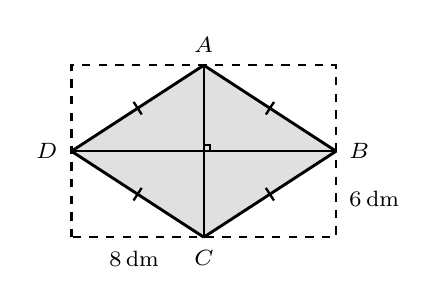
\begin{tikzpicture}[scale=0.42, every node/.style={font=\footnotesize, text=black}]
      \fill[white] (0,0) rectangle (8,5.2);
      \fill[gray!24] (4,0)--(8,2.6)--(4,5.2)--(0,2.6)--cycle;
      \draw[black, line width=0.85pt, dashed] (0,0) rectangle (8,5.2);
      \draw[black, line width=1.05pt, tk1] (4,0)--(8,2.6);
      \draw[black, line width=1.05pt, tk1] (8,2.6)--(4,5.2);
      \draw[black, line width=1.05pt, tk1] (4,5.2)--(0,2.6);
      \draw[black, line width=1.05pt, tk1] (0,2.6)--(4,0);
      \draw[black, line width=0.9pt] (0,2.6)--(8,2.6) (4,0)--(4,5.2);
      \rightbox[0.19cm]{4,5.2}{4,2.6}{8,2.6}
      \node[above=1pt] at (4,5.2) {$A$};
      \node[right=1.5pt] at (8,2.6) {$B$};
      \node[below=1pt] at (4,0) {$C$};
      \node[left=1.5pt] at (0,2.6) {$D$};
      \node[below=1.5pt] at (1.9,0) {$8\unit{dm}$};
      \node[right=1.5pt] at (8,1.15) {$6\unit{dm}$};
    \end{tikzpicture}
  \end{minipage}
\end{tcolorbox}

% ==================== ផ្នែកទី ២ ៖ E2 - EXPLORE ====================
\secbar{ផ្នែកទី ២ ៖ ការរុករកតាមស៊ុមចតុកោណកែងបំបែកត្រីកោណកែង ៨ (\enbf{E2 — Symmetry Frame})}{\en{11} នាទី (ពិភាក្សាដៃគូ)}

\begin{minipage}[c]{8.2cm}
  \centering
  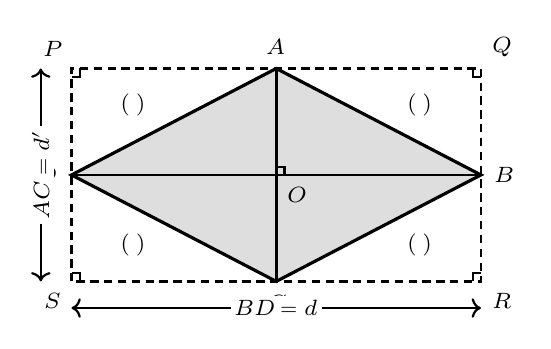
\begin{tikzpicture}[scale=0.52, every node/.style={font=\footnotesize, text=black}]
    \fill[white] (0,0) rectangle (10,5.2);
    \fill[gray!26] (5,0)--(10,2.6)--(5,5.2)--(0,2.6)--cycle;
    \draw[black, line width=0.95pt, densely dashed] (0,0) rectangle (10,5.2);
    \draw[black, line width=1.15pt] (5,0)--(10,2.6)--(5,5.2)--(0,2.6)--cycle;
    \draw[black, line width=0.95pt] (0,2.6)--(10,2.6) (5,0)--(5,5.2);
    \rightbox[0.20cm]{5,5.2}{5,2.6}{10,2.6}
    \rightbox[0.20cm]{0,2.6}{0,5.2}{5,5.2}
    \rightbox[0.20cm]{5,5.2}{10,5.2}{10,2.6}
    \rightbox[0.20cm]{10,2.6}{10,0}{5,0}
    \rightbox[0.20cm]{5,0}{0,0}{0,2.6}
    \node[above left=1pt] at (0,5.2) {$P$};
    \node[above right=1pt] at (10,5.2) {$Q$};
    \node[below right=1pt] at (10,0) {$R$};
    \node[below left=1pt] at (0,0) {$S$};
    \node[above=1.5pt] at (5,5.2) {$A$};
    \node[right=1.5pt] at (10,2.6) {$B$};
    \node[below=1.5pt] at (5,0) {$C$};
    \node[left=1.5pt] at (0,2.6) {$D$};
    \node[below right=1pt] at (5,2.6) {$O$};
    \node at (3.6,3.4) {\textbf{១}};
    \node at (6.4,3.4) {\textbf{២}};
    \node at (6.4,1.8) {\textbf{៣}};
    \node at (3.6,1.8) {\textbf{៤}};
    \node at (1.5,4.3) {(៥)};
    \node at (8.5,4.3) {(៦)};
    \node at (8.5,0.9) {(៧)};
    \node at (1.5,0.9) {(៨)};
    \draw[<->, black, line width=0.8pt] (0,-0.65) -- node[fill=white, inner sep=1.5pt] {$BD = d$} (10,-0.65);
    \draw[<->, black, line width=0.8pt] (-0.75,0) -- node[fill=white, inner sep=1.5pt, rotate=90] {$AC = d'$} (-0.75,5.2);
  \end{tikzpicture}
\end{minipage}\hfill
\begin{minipage}[c]{10.3cm}
  \textbf{សេចក្ដីណែនាំ៖} សង្កេតចតុកោណស្មើ $ABCD$ ដែលចារឹកក្នុងស៊ុមចតុកោណកែង $PQRS$ ខាងឆ្វេង រួចបំពេញចន្លោះ៖
  \begin{enumerate}[label=\textbf{\arabic*.}, leftmargin=1.4em, itemsep=2.5pt, topsep=2pt]
    \item ស៊ុមចតុកោណកែង $PQRS$ មានបណ្ដោយ $SR = BD =$ \blank{1.2cm} និងទទឹង $PS = AC =$ \blank{1.2cm} នាំឱ្យផ្ទៃក្រឡាស៊ុមធំ $S_{PQRS} =$ \blank{2.0cm}។
    \item ក្នុងការេតូចខាងឆ្វេងលើ $APOD$ បន្ទាត់ទ្រូង $AD$ ចែកវាជាត្រីកោណកែងពីរប៉ុនគ្នា គឺផ្នែក \textbf{១} និងផ្នែក \textbf{(៥)}។ ដូចគ្នាដែរ ក្នុងស៊ុមធំទាំងមូលមានត្រីកោណកែងប៉ុនគ្នាសរុបចំនួន \blank{1.2cm} ផ្នែក៖
    \begin{itemize}[leftmargin=1.2em, itemsep=1.5pt, topsep=1pt]
      \item ផ្នែកប្រផេះនៅក្នុងចតុកោណស្មើ $ABCD$ មានចំនួន \blank{1.2cm} ផ្នែក (១--៤)។
      \item ផ្នែកពណ៌សនៅក្រៅចតុកោណស្មើមានចំនួន \blank{1.2cm} ផ្នែក (៥--៨)។
    \end{itemize}
    \item ដូចនេះ ផ្ទៃចតុកោណស្មើ $ABCD$ ស្មើនឹងប្រភាគ $\dfrac{\blank{0.8cm}}{8} =$ \blank{1.0cm} នៃផ្ទៃស៊ុម $PQRS$ គឺ៖ $\mathbf{S_{ABCD} =}$ \blank{3.0cm}។
    \item \textbf{អន្ទាក់ការយល់ច្រឡំទី១៖} បើគេគណនា $d \times d'$ ដោយភ្លេចចែកនឹង $2$ តើគេកំពុងគណនាផ្ទៃអ្វី? ចម្លើយ៖ \blank{4.0cm}។
  \end{enumerate}
\end{minipage}

\vspace{3pt}
\begin{tcolorbox}[
  enhanced, sharp corners, colback=panelgray, colframe=black,
  boxrule=0.85pt, boxsep=2pt, top=3pt, bottom=3pt, left=6pt, right=6pt, after skip=3pt
]
  \textbf{5. អន្ទាក់ការយល់ច្រឡំទី២ (ប្រៀបធៀប «អង្កត់ទ្រូងពេញ» ទល់នឹង «កន្លះអង្កត់ទ្រូង»)៖}
  \begin{itemize}[leftmargin=1.3em, itemsep=2pt, topsep=1.5pt]
    \item \textbf{ករណី ក៖} បើប្រាប់អង្កត់ទ្រូងពេញ $AC = d = 12\unit{cm}$ និង $BD = d' = 8\unit{cm}$ នោះ $S = \dfrac{1}{2} \times$ \blank{1.2cm} $\times$ \blank{1.2cm} $=$ \blank{1.6cm} $\unit{cm}^2$។
    \item \textbf{ករណី ខ៖} បើរូបភាពប្រាប់កន្លះអង្កត់ទ្រូង $OA = 6\unit{cm}$ និង $OB = 4\unit{cm}$ ត្រូវរកអង្កត់ទ្រូងពេញសិន៖ $d = 2 \times 6 =$ \blank{1.2cm} $\unit{cm}$ និង $d' = 2 \times 4 =$ \blank{1.2cm} $\unit{cm} \Rightarrow S =$ \blank{1.6cm} $\unit{cm}^2$ (ហាមយក $\frac{1}{2}\times 6\times 4 = 12\unit{cm}^2$ ដាច់ខាត!)។
  \end{itemize}
\end{tcolorbox}

% ==================== ផ្នែកទី ៣ ៖ E3 - EXPLAIN ====================
\secbar{ផ្នែកទី ៣ ៖ សំយោគទ្រឹស្ដីបទ សម្រាយបញ្ជាក់ផ្លូវការ និងធនាគារហេតុផល (\enbf{E3 — Explain})}{\en{6} នាទី (ទំ.១៩០)}

\begin{tcolorbox}[
  enhanced, sharp corners, colback=white, colframe=black,
  boxrule=1.0pt, boxsep=2pt, top=3.5pt, bottom=3.5pt, left=6pt, right=6pt
]
  \begin{minipage}[c]{12.6cm}
    $\bullet$ \textbf{ទ្រឹស្ដីបទ (ទំ.១៩០)៖} ផ្ទៃក្រឡាចតុកោណស្មើដែលមានអង្កត់ទ្រូងទាំងពីរ $d$ និង $d'$ កំណត់ដោយរូបមន្ត៖ $\mathbf{S =}$ \blank{2.6cm} ។\\[2.5pt]
    $\bullet$ \textbf{សម្រាយបញ្ជាក់តាមការបូកត្រីកោណពីរ (ទំ.១៩០)៖} អង្កត់ទ្រូង $BD = d'$ ចែក $ABCD$ ជាត្រីកោណ $\tri{ABD}$ និង $\tri{CBD}$ ដែលមានកម្ពស់កែង $AO$ និង $CO$ ($AC \perp BD$)៖\\[2pt]
    \hspace*{0.3cm}$S_{ABCD} = S_{\tri{ABD}} + S_{\tri{CBD}} = \dfrac{1}{2} BD \cdot$ \blank{1.1cm} $+ \dfrac{1}{2} BD \cdot$ \blank{1.1cm}\\
    \hspace*{1.48cm}$= \dfrac{1}{2} BD ($ \blank{2.0cm} $) = \dfrac{1}{2} BD \cdot$ \blank{1.1cm} $=$ \blank{2.0cm} ។
  \end{minipage}\hfill
  \begin{minipage}[c]{5.6cm}
    \centering
    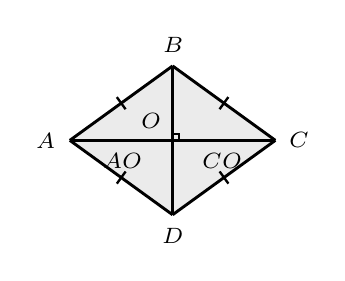
\begin{tikzpicture}[scale=0.45, every node/.style={font=\footnotesize, text=black}]
      \coordinate (A) at (0,2.1);
      \coordinate (B) at (2.9,4.2);
      \coordinate (C) at (5.8,2.1);
      \coordinate (D) at (2.9,0);
      \coordinate (O) at (2.9,2.1);
      \fill[gray!16] (A)--(B)--(C)--(D)--cycle;
      \draw[black, line width=1.05pt, tk1] (A)--(B);
      \draw[black, line width=1.05pt, tk1] (B)--(C);
      \draw[black, line width=1.05pt, tk1] (C)--(D);
      \draw[black, line width=1.05pt, tk1] (D)--(A);
      \draw[black, line width=0.9pt] (A)--(C) (B)--(D);
      \rightbox[0.19cm]{B}{O}{C}
      \node[left=1.5pt] at (A) {$A$};
      \node[above=1.5pt] at (B) {$B$};
      \node[right=1.5pt] at (C) {$C$};
      \node[below=1.5pt] at (D) {$D$};
      \node[above left=1pt] at (O) {$O$};
      \node[below=1pt] at (1.50,2.1) {$AO$};
      \node[below=1pt] at (4.30,2.1) {$CO$};
    \end{tikzpicture}
  \end{minipage}\\[4pt]
  \begin{tabular}{|p{4.3cm}|p{3.8cm}|p{4.3cm}|p{4.8cm}|}
    \hline
    \cellcolor{headgray}\centering\textbf{\cnum{1} លក្ខណៈអង្កត់ទ្រូង} &
    \cellcolor{headgray}\centering\textbf{\cnum{2} រូបមន្តផ្ទាល់} &
    \cellcolor{headgray}\centering\textbf{\cnum{3} រូបមន្តច្រាសរក $d'$} &
    \cellcolor{headgray}\centering\arraybackslash\textbf{\cnum{4} ទំនាក់ទំនងជ្រុង $a$} \\[2pt]
    \hline
    $AC \perp BD$ ត្រង់ $O$ ហើយ $OA = \frac{d}{2},\; OB = \frac{d'}{2}$ &
    \centering $S = \dfrac{1}{2} d \times d'$ &
    \centering $2S = d \cdot d' \Rightarrow d' = \dfrac{2S}{d}$ &
    \centering\arraybackslash ក្នុង $\tri{AOB}$៖ $a^2 = \left(\frac{d}{2}\right)^2 + \left(\frac{d'}{2}\right)^2$ \par និង $S = a \times h$ \\[2pt]
    \hline
  \end{tabular}
\end{tcolorbox}

\newpage

% ==================== ទំព័រទី ២ ៖ E4, E5 និងកិច្ចការផ្ទះ ====================
\secbar{ផ្នែកទី ៤ ៖ លំហាត់គំរូថយជំនួយតាមជំហាន (\enbf{E4 — Backward-Faded Worked Examples})}{\en{10} នាទី (ទំ.១៩០--១៩១)}

\begin{tcolorbox}[
  enhanced, sharp corners, colback=white, colframe=black,
  boxrule=0.95pt, boxsep=2pt, top=4pt, bottom=4pt, left=6pt, right=6pt, after skip=5pt
]
  \begin{minipage}[c]{12.0cm}
    \textbf{លំហាត់គំរូទី ១ (ទំ.១៩០ — គណនាផ្ទៃក្រឡាផ្ទាល់)៖}\\
    រកផ្ទៃក្រឡានៃចតុកោណស្មើមួយ ដែលមានរង្វាស់អង្កត់ទ្រូង $d = 13\unit{cm}$ និង $d' = 14\unit{cm}$។\\[2.5pt]
    $\bullet$ \textbf{ជំហានទី ១ (ពិនិត្យទិន្នន័យ)៖} តើ $13\unit{cm}$ និង $14\unit{cm}$ ជាកន្លះអង្កត់ទ្រូង ឬអង្កត់ទ្រូងពេញ? \blank{2.8cm}\\[2.5pt]
    $\bullet$ \textbf{ជំហានទី ២ (ជំនួសក្នុង \cnum{2} រួចសម្រួលមុនគុណ)៖}\\
    \hspace*{0.5cm}$S = \dfrac{d \times d'}{2} = \dfrac{\blank{1.4cm} \times \blank{1.4cm}}{2} = 13 \times$ \blank{1.3cm} $=$ \blank{1.8cm} $\unit{cm}^2$។\\[2.5pt]
    $\bullet$ \textbf{ពិនិត្យឯកតា៖} បើអង្កត់ទ្រូងគិតជា $\unit{cm}$ នោះផ្ទៃក្រឡាត្រូវគិតជា \blank{1.8cm}។
  \end{minipage}\hfill
  \begin{minipage}[c]{6.2cm}
    \centering
    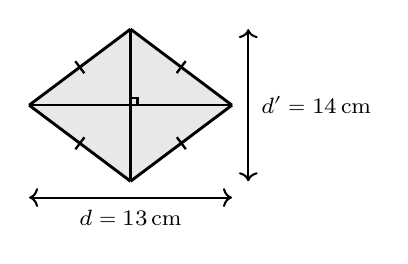
\begin{tikzpicture}[scale=0.46, every node/.style={font=\footnotesize, text=black}]
      \coordinate (A) at (0,2.1);
      \coordinate (B) at (2.8,4.2);
      \coordinate (C) at (5.6,2.1);
      \coordinate (D) at (2.8,0);
      \coordinate (O) at (2.8,2.1);
      \fill[gray!18] (A)--(B)--(C)--(D)--cycle;
      \draw[black, line width=1.05pt, tk1] (A)--(B);
      \draw[black, line width=1.05pt, tk1] (B)--(C);
      \draw[black, line width=1.05pt, tk1] (C)--(D);
      \draw[black, line width=1.05pt, tk1] (D)--(A);
      \draw[black, line width=0.9pt] (A)--(C) (B)--(D);
      \rightbox[0.19cm]{B}{O}{C}
      \draw[<->, black, line width=0.75pt] (0,-0.45) -- node[below=1pt] {$d=13\unit{cm}$} (5.6,-0.45);
      \draw[<->, black, line width=0.75pt] (6.05,0) -- node[right=1pt] {$d'=14\unit{cm}$} (6.05,4.2);
    \end{tikzpicture}
  \end{minipage}
\end{tcolorbox}

\begin{tcolorbox}[
  enhanced, sharp corners, colback=panelgray, colframe=black,
  boxrule=0.95pt, boxsep=2pt, top=4pt, bottom=4pt, left=6pt, right=6pt, after skip=5pt
]
  \begin{minipage}[c]{12.0cm}
    \textbf{លំហាត់គំរូទី ២ (ទំ.១៩១ — រកអង្កត់ទ្រូងបាត់តាមរូបមន្តច្រាស)៖}\\
    ចតុកោណស្មើមួយមានផ្ទៃក្រឡាស្មើនឹង $1000\unit{mm}^2$ និងមានរង្វាស់អង្កត់ទ្រូងមួយស្មើនឹង $10\unit{mm}$។ គណនារង្វាស់អង្កត់ទ្រូងមួយទៀត $d'$។\\[2.5pt]
    $\bullet$ \textbf{ជំហានទី ១ (បំបាត់ភាគបែង $2$ តាម \cnum{3})៖} ពី $S = \dfrac{d \times d'}{2} \implies d \times d' = 2 \times S = 2 \times$ \blank{1.6cm} $=$ \blank{1.8cm}\\[2.5pt]
    $\bullet$ \textbf{ជំហានទី ២ (ទាញរក $d'$)៖} $d' = \dfrac{2S}{d} = \dfrac{\blank{1.8cm}}{\blank{1.4cm}} =$ \blank{2.0cm} $\unit{mm}$ ($=$ \blank{1.4cm} $\unit{cm}$)។\\[2.5pt]
    $\bullet$ \textbf{ពន្យល់ខ្លួនឯង (\en{Self-Explanation})៖} ហេតុអ្វីចម្លើយ $1000 \div 10 = 100\unit{mm}$ \textbf{ខុស}? \blank{4.4cm}
  \end{minipage}\hfill
  \begin{minipage}[c]{6.2cm}
    \centering
    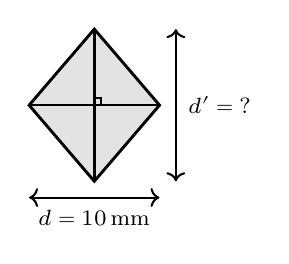
\begin{tikzpicture}[scale=0.46, every node/.style={font=\footnotesize, text=black}]
      \coordinate (A) at (1.0,2.1);
      \coordinate (B) at (2.8,4.2);
      \coordinate (C) at (4.6,2.1);
      \coordinate (D) at (2.8,0);
      \coordinate (O) at (2.8,2.1);
      \fill[gray!22] (A)--(B)--(C)--(D)--cycle;
      \draw[black, line width=1.05pt] (A)--(B)--(C)--(D)--cycle;
      \draw[black, line width=0.9pt] (A)--(C) (B)--(D);
      \rightbox[0.19cm]{B}{O}{C}
      \draw[<->, black, line width=0.75pt] (1.0,-0.45) -- node[below=1pt] {$d=10\unit{mm}$} (4.6,-0.45);
      \draw[<->, black, line width=0.75pt] (5.05,0) -- node[right=1pt] {$d'=?$} (5.05,4.2);
    \end{tikzpicture}
  \end{minipage}
\end{tcolorbox}

% ==================== ផ្នែកទី ៥ ៖ E5 - EVALUATE ====================
\secbar{ផ្នែកទី ៥ ៖ លំហាត់ប្រតិបត្តិ និងវាយតម្លៃរហ័ស (\enbf{E5 — Think-Pair-Check \& Exit Check})}{\en{10} នាទី (ទំ.១៩១)}

\noindent
\begin{minipage}[t]{10.5cm}
  \begin{tcolorbox}[
    enhanced, sharp corners, colback=white, colframe=black,
    boxrule=0.95pt, boxsep=2pt, top=4pt, bottom=4pt, left=5pt, right=5pt, equal height group=e5area2
  ]
    \textbf{១. ប្រតិបត្តិ (ទំ.១៩១)៖} ចតុកោណស្មើ $ABCD$ មានផ្ទៃក្រឡា $S = 120\unit{cm}^2$ និងអង្កត់ទ្រូងវែង $AC = d = 30\unit{cm}$។
    \begin{center}
      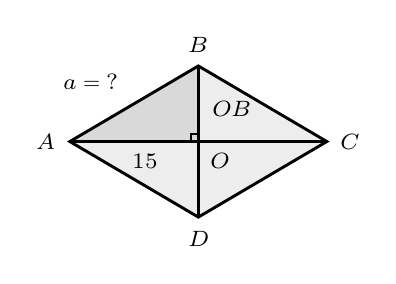
\begin{tikzpicture}[scale=0.48, every node/.style={font=\footnotesize, text=black}]
        \coordinate (A) at (0,2.0);
        \coordinate (B) at (3.4,4.0);
        \coordinate (C) at (6.8,2.0);
        \coordinate (D) at (3.4,0);
        \coordinate (O) at (3.4,2.0);
        \fill[gray!14] (A)--(B)--(C)--(D)--cycle;
        \fill[gray!30] (A)--(O)--(B)--cycle;
        \draw[black, line width=1.05pt] (A)--(B)--(C)--(D)--cycle;
        \draw[black, line width=0.9pt] (A)--(C) (B)--(D);
        \rightbox[0.19cm]{B}{O}{A}
        \node[left=1.5pt] at (A) {$A$};
        \node[above=1.5pt] at (B) {$B$};
        \node[right=1.5pt] at (C) {$C$};
        \node[below=1.5pt] at (D) {$D$};
        \node[below right=1pt] at (O) {$O$};
        \node[below=1pt] at (2.0,2.0) {$15$};
        \node[right=1.5pt] at (3.4,2.85) {$OB$};
        \node[above left=1pt] at (1.6,3.05) {$a=?$};
      \end{tikzpicture}
    \end{center}
    \textbf{ក.} រកអង្កត់ទ្រូងខ្លី $BD = d' = \dfrac{2S}{d} = \dfrac{2 \times \blank{1.3cm}}{\blank{1.3cm}} =$ \blank{1.5cm} $\unit{cm}$\\[3pt]
    \textbf{ខ.} ក្នុង $\tri{AOB}$ កែងត្រង់ $O$ មាន $OA = 15\unit{cm}$ និង $OB = \frac{d'}{2} =$ \blank{1.1cm} $\unit{cm}$\\
    \hspace*{0.4cm}ជ្រុង $a = \sqrt{OA^2 + OB^2} = \sqrt{\blank{1.3cm} + \blank{1.1cm}} = \sqrt{\blank{1.3cm}} \approx$ \blank{1.5cm} $\unit{cm}$\\[2.5pt]
    \chkbox\ \textit{បានផ្ទៀងផ្ទាត់ជាមួយដៃគូរួចរាល់}
  \end{tcolorbox}
\end{minipage}\hfill
\begin{minipage}[t]{8.2cm}
  \begin{tcolorbox}[
    enhanced, sharp corners, colback=white, colframe=black,
    boxrule=0.95pt, boxsep=2pt, top=4pt, bottom=4pt, left=5pt, right=5pt, equal height group=e5area2
  ]
    \textbf{២. តេស្តរហ័ស ៩០ វិនាទី (\en{Exit Check})៖} ចតុកោណស្មើខាងក្រោមមានកន្លះអង្កត់ទ្រូង $OA = 5\unit{cm}$ និង $OB = 4\unit{cm}$៖
    \begin{center}
      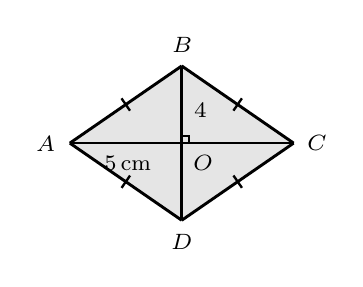
\begin{tikzpicture}[scale=0.49, every node/.style={font=\footnotesize, text=black}]
        \coordinate (A) at (0,2.0);
        \coordinate (B) at (2.9,4.0);
        \coordinate (C) at (5.8,2.0);
        \coordinate (D) at (2.9,0);
        \coordinate (O) at (2.9,2.0);
        \fill[gray!20] (A)--(B)--(C)--(D)--cycle;
        \draw[black, line width=1.05pt, tk1] (A)--(B);
        \draw[black, line width=1.05pt, tk1] (B)--(C);
        \draw[black, line width=1.05pt, tk1] (C)--(D);
        \draw[black, line width=1.05pt, tk1] (D)--(A);
        \draw[black, line width=0.9pt] (A)--(C) (B)--(D);
        \rightbox[0.19cm]{B}{O}{C}
        \node[left=1.5pt] at (A) {$A$};
        \node[above=1.5pt] at (B) {$B$};
        \node[right=1.5pt] at (C) {$C$};
        \node[below=1.5pt] at (D) {$D$};
        \node[below right=1pt] at (O) {$O$};
        \node[below=1pt] at (1.50,2.0) {$5\unit{cm}$};
        \node[right=1pt] at (2.9,2.85) {$4$};
      \end{tikzpicture}
    \end{center}
    តើផ្ទៃក្រឡា $S_{ABCD}$ ស្មើនឹងប៉ុន្មាន? (គូសធីកតែ ១)៖\\[2pt]
    \chkbox\ \textbf{A.} $10\unit{cm}^2$ \hspace{0.9cm} \chkbox\ \textbf{B.} $20\unit{cm}^2$\\[2.5pt]
    \chkbox\ \textbf{C.} $40\unit{cm}^2$ \hspace{0.9cm} \chkbox\ \textbf{D.} $80\unit{cm}^2$\\[3pt]
    \textbf{បិទបេសកកម្ម E1៖} ផ្ទៃខ្លែង $S =$ \blank{1.9cm} $\unit{dm}^2$។
  \end{tcolorbox}
\end{minipage}

% ==================== កិច្ចការផ្ទះ (ជំហានទី ៥) ====================
\vspace{4pt}
\begin{tcolorbox}[
  enhanced, sharp corners, colback=panelgray, colframe=black,
  boxrule=1.0pt, boxsep=2pt, top=3.5pt, bottom=3.5pt, left=6pt, right=6pt
]
  {\muol\fontsize{9.0pt}{13pt}\selectfont កិច្ចការផ្ទះ (សៀវភៅសិក្សាគោល ទំព័រ ១៩៥ — ធ្វើដាក់ក្នុងសៀវភៅលំហាត់សម្រាប់ម៉ោងក្រោយ)}\\[2pt]
  $\bullet$ \textbf{លំហាត់ទី ៧ រូបចតុកោណស្មើខាងឆ្វេង (ទំ.១៩៥)៖} គណនាផ្ទៃក្រឡា និងបរិមាត្រចតុកោណស្មើដែលមានជ្រុង $4.0$ និងអង្កត់ទ្រូងទាំងពីរ $4.5$ និង $6.7$។\\
  $\bullet$ \textbf{លំហាត់ទី ៧ រូបចតុកោណស្មើខាងស្ដាំ (ទំ.១៩៥)៖} គណនាផ្ទៃក្រឡា និងបរិមាត្រចតុកោណស្មើដែលមានជ្រុង $32$ និងអង្កត់ទ្រូងទាំងពីរ $50$ និង $40$។ \textit{(អានមុន៖ ចំណុច ៣. ផ្ទៃក្រឡាចតុកោណព្នាយ ទំ.១៩១--១៩៣)}
\end{tcolorbox}

\end{document}
